\chapter{Benchmarking and Experiments}
\label{chapter5}
% Introduce each domain, what makes it difficult, why it was chosen, etc. Show results from each domain, and discuss.
% \cite{osband2020bsuite, 1606.01540}
% \section{Deterministic Gridworld}
% A simple gridworld, with a door that is open. The model embedded has a closed door.
% \section{Stochastic Gridworld}
% A simple gridworld, with a door that is open with probability 0.5, closed otherwise. The model embedded suggests that the door is closed with probability 1.0.
% \section{Cliff-Walking}
% \begin{figure}[h!]
%     \centering
%     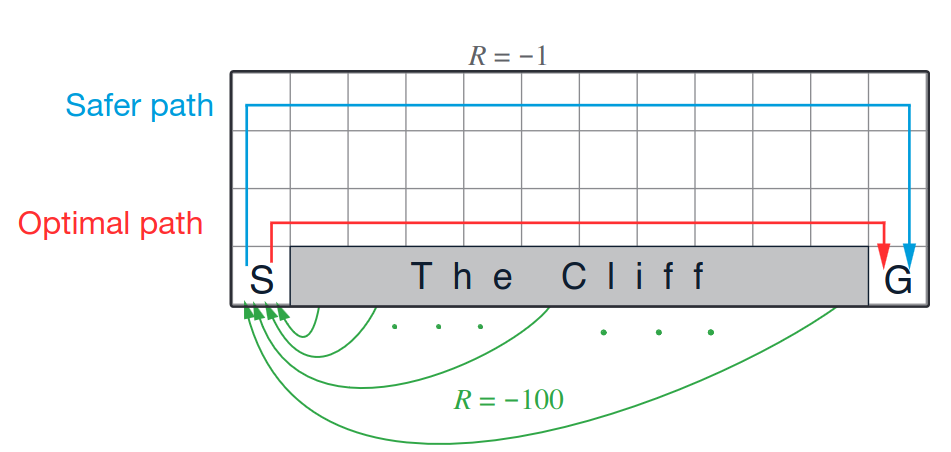
\includegraphics[max size={\textwidth}{\textheight}]{report/assets/envs/cliff-walking.png}
%     \caption{Cliff-Walking Environment \cite{Sutton1998}}
%     \label{fig:cliff-walking}
% \end{figure}
% \cite{1606.01540, Sutton1998}
% \section{Windy Gridworld}
% \begin{figure}[h!]
%     \centering
%     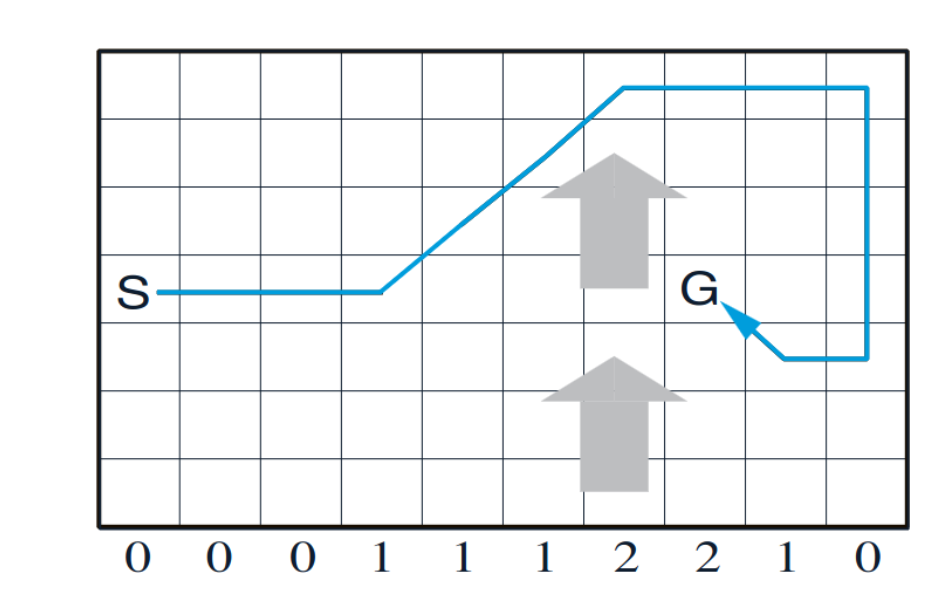
\includegraphics[max size={\textwidth}{\textheight}]{report/assets/envs/windy.png}
%     \caption{Windy GridWorld Environment \cite{Sutton1998}}
%     \label{fig:windy}
% \end{figure}
% \cite{Sutton1998}
% \section{Stochastic Windy Gridworld}
% \section{Frozen Lake}
% \begin{figure}[h!]
%     \centering
%     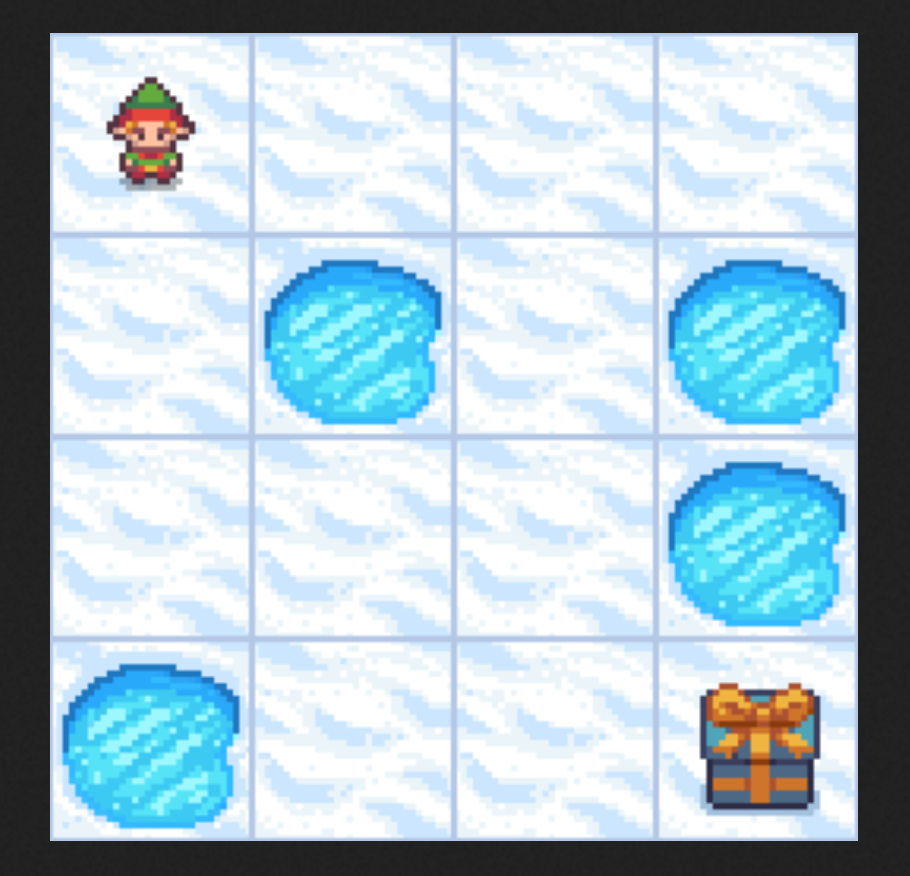
\includegraphics[max size={\textwidth}{\textheight}]{report/assets/envs/frozen-lake.png}
%     \caption{Frozen Lake Environment \cite{1606.01540}}
%     \label{fig:frozen}
% \end{figure}
% \cite{1606.01540}
% \section{Discrete Cart-Pole}
% \begin{figure}[h!]
%     \centering
%     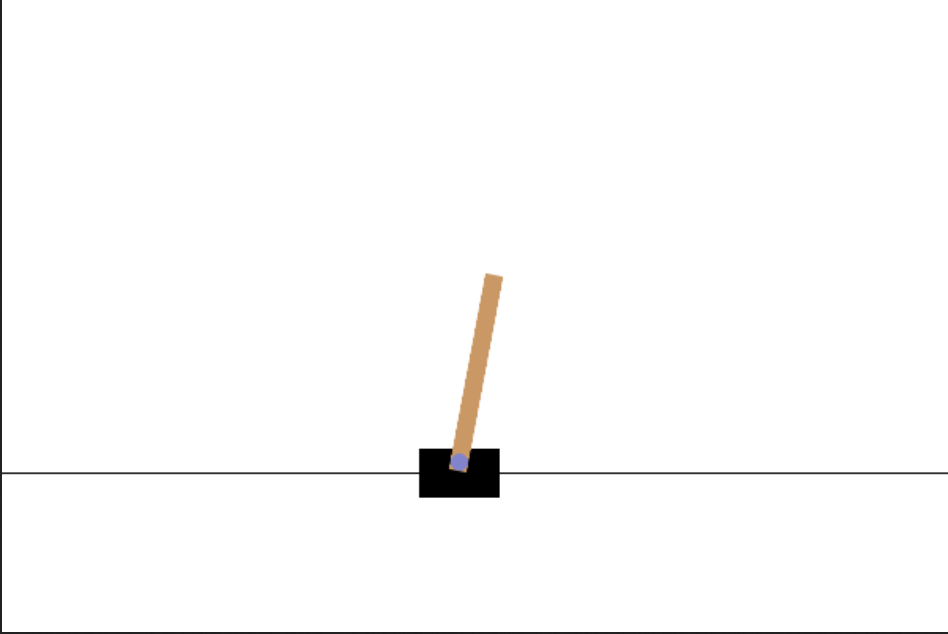
\includegraphics[max size={\textwidth}{\textheight}]{report/assets/envs/cartpole.png}
%     \caption{CartPole Environment \cite{1606.01540, 6313077}}
%     \label{fig:cartpole}
% \end{figure}
% \cite{1606.01540, 6313077}
% \section{Discrete Mountain Car}
% \begin{figure}[h!]
%     \centering
%     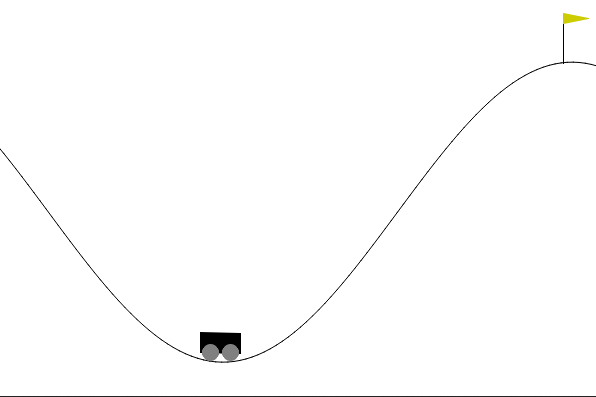
\includegraphics[max size={\textwidth}{\textheight}]{report/assets/envs/mountaincar.png}
%     \caption{Mountain Car Environment \cite{1606.01540, Moore90efficientmemory-based}}
%     \label{fig:cartpole}
% \end{figure}
% \cite{1606.01540, Moore90efficientmemory-based}